% !TeX root = ../main.tex
% Add the above to each chapter to make compiling the PDF easier in some editors.

\chapter{Results}\label{chapter:results}
\section{Depth Completion Performance}

The evaluation of our depth completion model was conducted using 25 test images from the ``Leaves on the Ground'' scenario that is introduced in Table \ref{table:scenariosobjectmodification} in our simulated environment. To assess the model's performance, we employed two widely-used metrics in depth completion tasks: \ac{MAE} and inverse \ac{iRMSE}.

\ac{MAE} provides a direct measure of the average deviation between predicted and ground truth depth values. This metric is particularly valuable for understanding the absolute accuracy of depth predictions across the entire scene. \ac{iRMSE}, calculated using inverse depth values, places greater emphasis on accuracy in closer ranges - a crucial consideration for \ac{AV} applications where precise depth estimation of nearby objects is essential for safe navigation.

Our evaluation yielded the following results:
\begin{table}[h]
\centering
\begin{tabular}{ll}
\hline
\textbf{Metric} & \textbf{Value} \\
\hline
Average \ac{MAE} & 744.4308 \\
Average \ac{iRMSE} & 47.7721 \\
Inference Time & 70-75 ms on NVIDIA RTX4090 \\
\hline
\end{tabular}
\caption{Performance metrics of the depth completion model}
\label{tab:depth_metrics}
\end{table}

While these metrics appear less favorable compared to state-of-the-art results on the KITTI benchmark (\ac{MAE}: 192.71, \ac{iRMSE}: 1.88), direct comparisons would be misleading due to fundamental differences in data domain, depth representation, and training strategy between our implementation and the KITTI benchmark. Table \ref{tab:implementation_differences} highlights key distinctions between our implementation and the KITTI benchmark.

\begin{table}[h]
\centering
\begin{tabular}{p{0.3\textwidth}p{0.6\textwidth}}
\hline
\textbf{Aspect} & \textbf{Difference} \\
\hline
Data Domain & Our implementation uses simulated data from CARLA's depth camera, whereas KITTI employs real-world \ac{LiDAR} data with different characteristics and challenges \\
Depth Representation & Our model operates on grayscale depth maps with values ranging from 0-255, while KITTI uses metric depth measurements \\
Training Strategy & We employed masked training that explicitly excludes sky regions and distant objects, as evidenced by the black regions in Figure~\ref{fig:depth_pred} \\
\hline
\end{tabular}
\caption{Key differences between our implementation and KITTI benchmark}
\label{tab:implementation_differences}
\end{table}

\subsection{Limitations and Context of Performance Metrics}

The reported metrics should be interpreted within the specific context of our research objectives. While these numerical values provide quantitative measures of the model's performance, their significance is limited without comparative benchmarks against alternative implementations or different architectural approaches.

Given that our primary research focus is on human-machine interaction rather than optimizing depth completion algorithms, we prioritized developing a functionally adequate model that serves our experimental needs. Our hypothesis is that the depth completion component, as shown in Figure~\ref{fig:depth_model_comparison}, provides sufficient depth information for our human-machine interaction studies, despite potential room for improvement in absolute accuracy.

In our user study, we specifically examined the practical impact of our depth completion model by comparing user experience and performance between:

\begin{table}[h]
\centering
\begin{tabular}{ll}
\hline
\textbf{Scenario} & \textbf{Description} \\
\hline
Current Implementation & With its inherent imperfections \\
Perfect Depth Information & Ideal depth information scenarios \\
\hline
\end{tabular}
\caption{Comparison scenarios in user study}
\label{tab:comparison_scenarios}
\end{table}

This comparative approach aligns with our research goals of understanding how depth completion quality affects human-machine interaction, rather than achieving state-of-the-art depth completion performance. The development and evaluation of more sophisticated depth completion models, including comprehensive comparisons with alternative approaches, remains an opportunity for future research beyond the scope of this thesis.

\begin{figure}[h]
    \centering
    \begin{subfigure}{0.48\textwidth}
        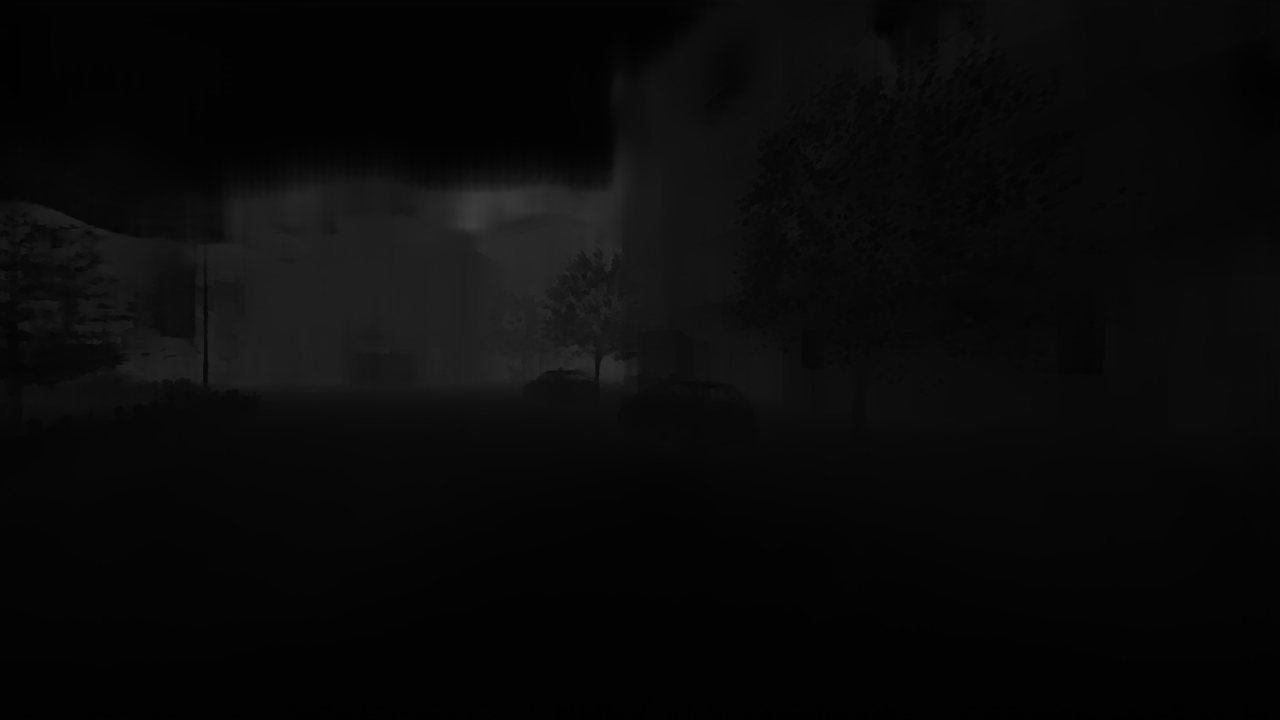
\includegraphics[width=\textwidth]{figures/depth_pred.png}
        \caption{Model output}
        \label{fig:depth_pred}
    \end{subfigure}
    \hfill
    \begin{subfigure}{0.48\textwidth}
        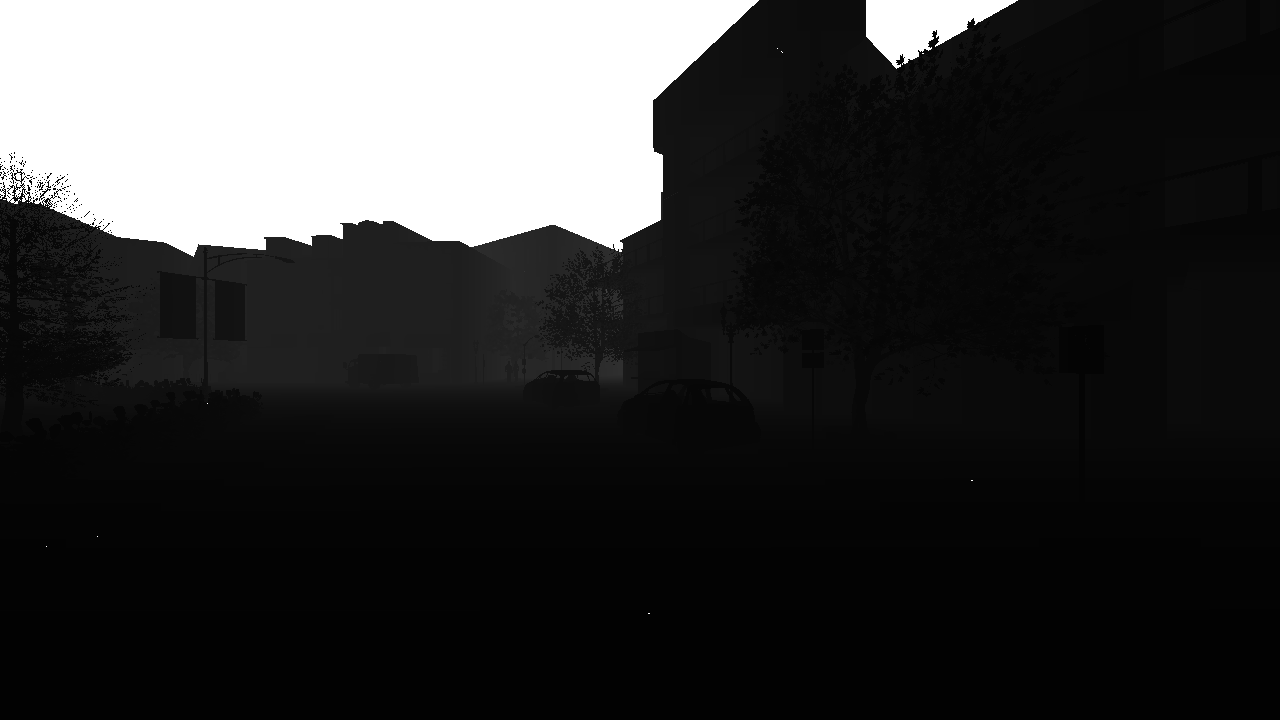
\includegraphics[width=\textwidth]{figures/depth_gt_2.png}
        \caption{Ground truth}
        \label{fig:depth_gt_2}
    \end{subfigure}
    \caption{Depth completion model output compared to ground truth}
    \label{fig:depth_model_comparison}
    \end{figure}


\section{Interface Comparison}

Following the implementation of our three interface variants, we conducted a technical comparison to evaluate their capabilities and performance characteristics. Each interface represents a distinct approach to visualizing teleoperation data:

\subsection*{Separate View}

The Separate View follows the traditional teleoperation interface design principles outlined in Section \ref{section:separateview}. Our implementation enhances the base variant by incorporating \ac{LiDAR} point cloud coloring for improved depth perception and environmental understanding. As shown in Figure \ref{fig:res_sv}, the interface maintains distinct windows for 2D camera feeds and 3D perception data, aligning with established industry approaches like in Figures \ref{fig:Waymo} and \ref{fig:Zoox}.

This variant's key technical advantage lies in its deterministic nature, operating without reliance on deep learning models. The visualization outcome depends solely on direct sensor inputs and rendering processes, making it particularly robust across diverse environments. The absence of learned components provides two significant benefits:
\paragraph{Environmental Adaptability}
The interface maintains consistent performance even in previously unseen scenarios, as it doesn't depend on training data distributions.
\paragraph{View Flexibility}
The point cloud representation maintains accuracy within sensor error bounds when viewed from multiple angles, unlike estimation-based approaches where small errors can compound into visible artifacts during perspective shifts.

These technical characteristics make the Separate View particularly suitable for scenarios requiring high reliability and precise spatial understanding, though at the cost of maintaining multiple display windows.
\begin{figure}[h]
    \centering
    \begin{subfigure}{0.8\textwidth}
        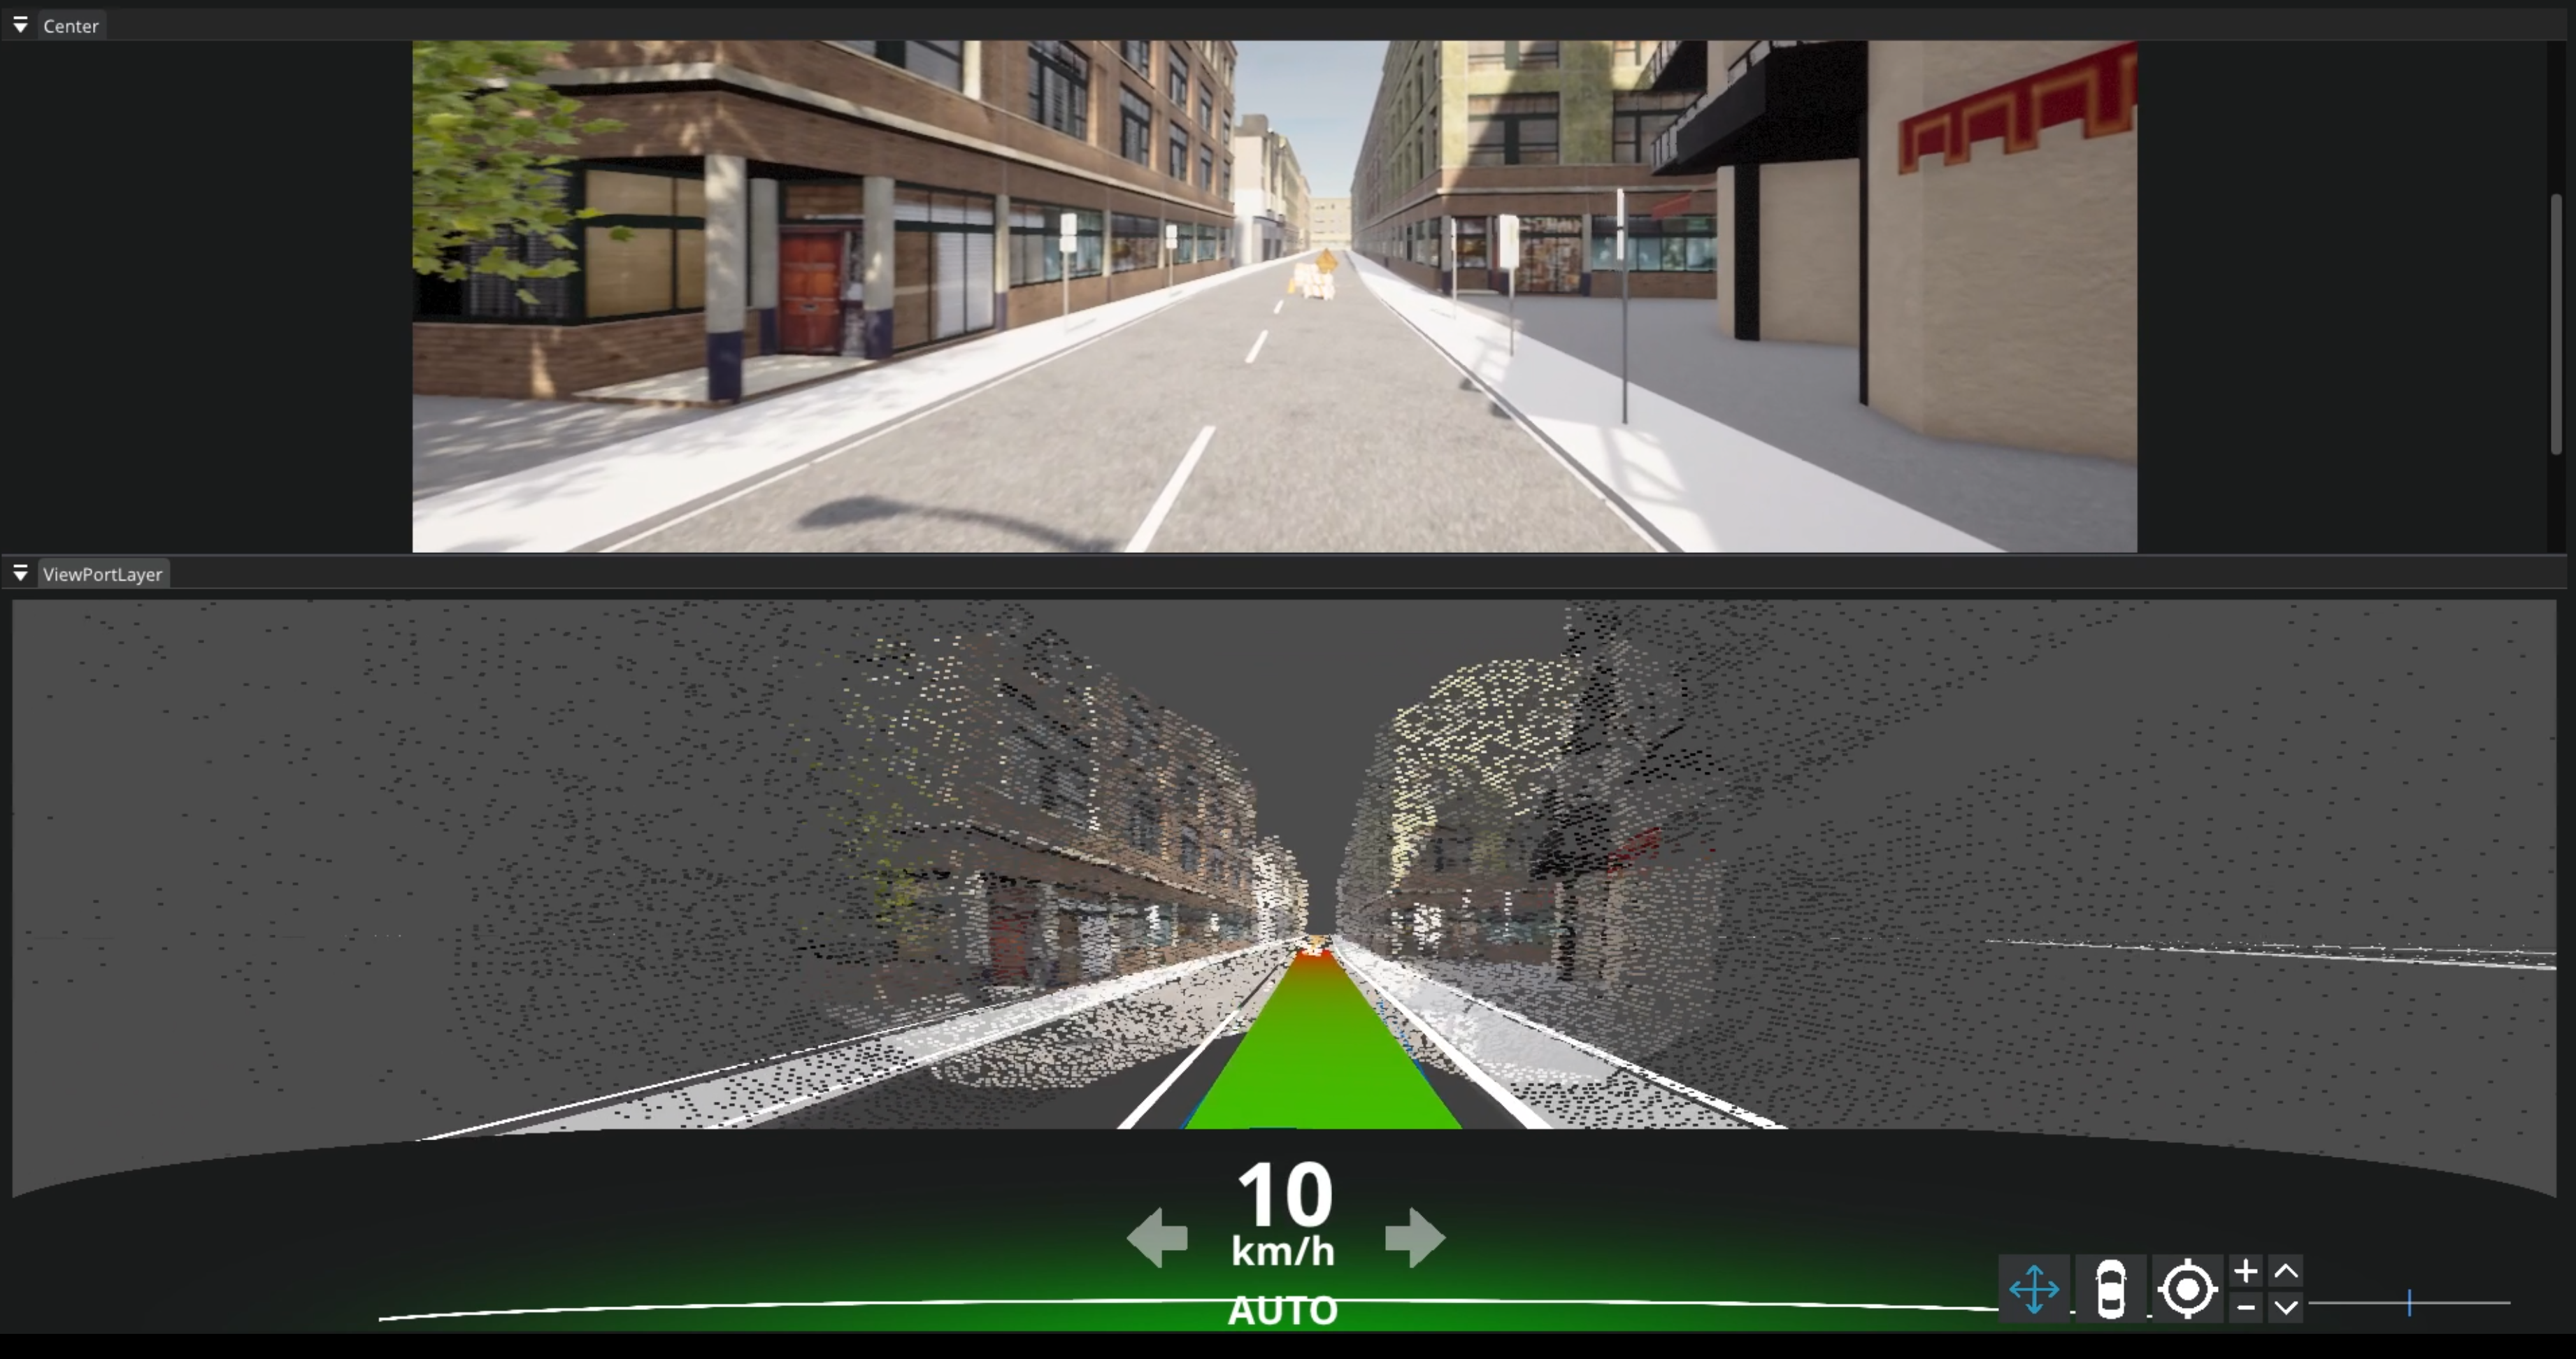
\includegraphics[width=\textwidth]{figures/result_sv.png}
        \centering
        \caption{Separate View Interface before a construction site}
        \label{fig:res_sv_1}
    \end{subfigure}
    \begin{subfigure}{0.8\textwidth}
        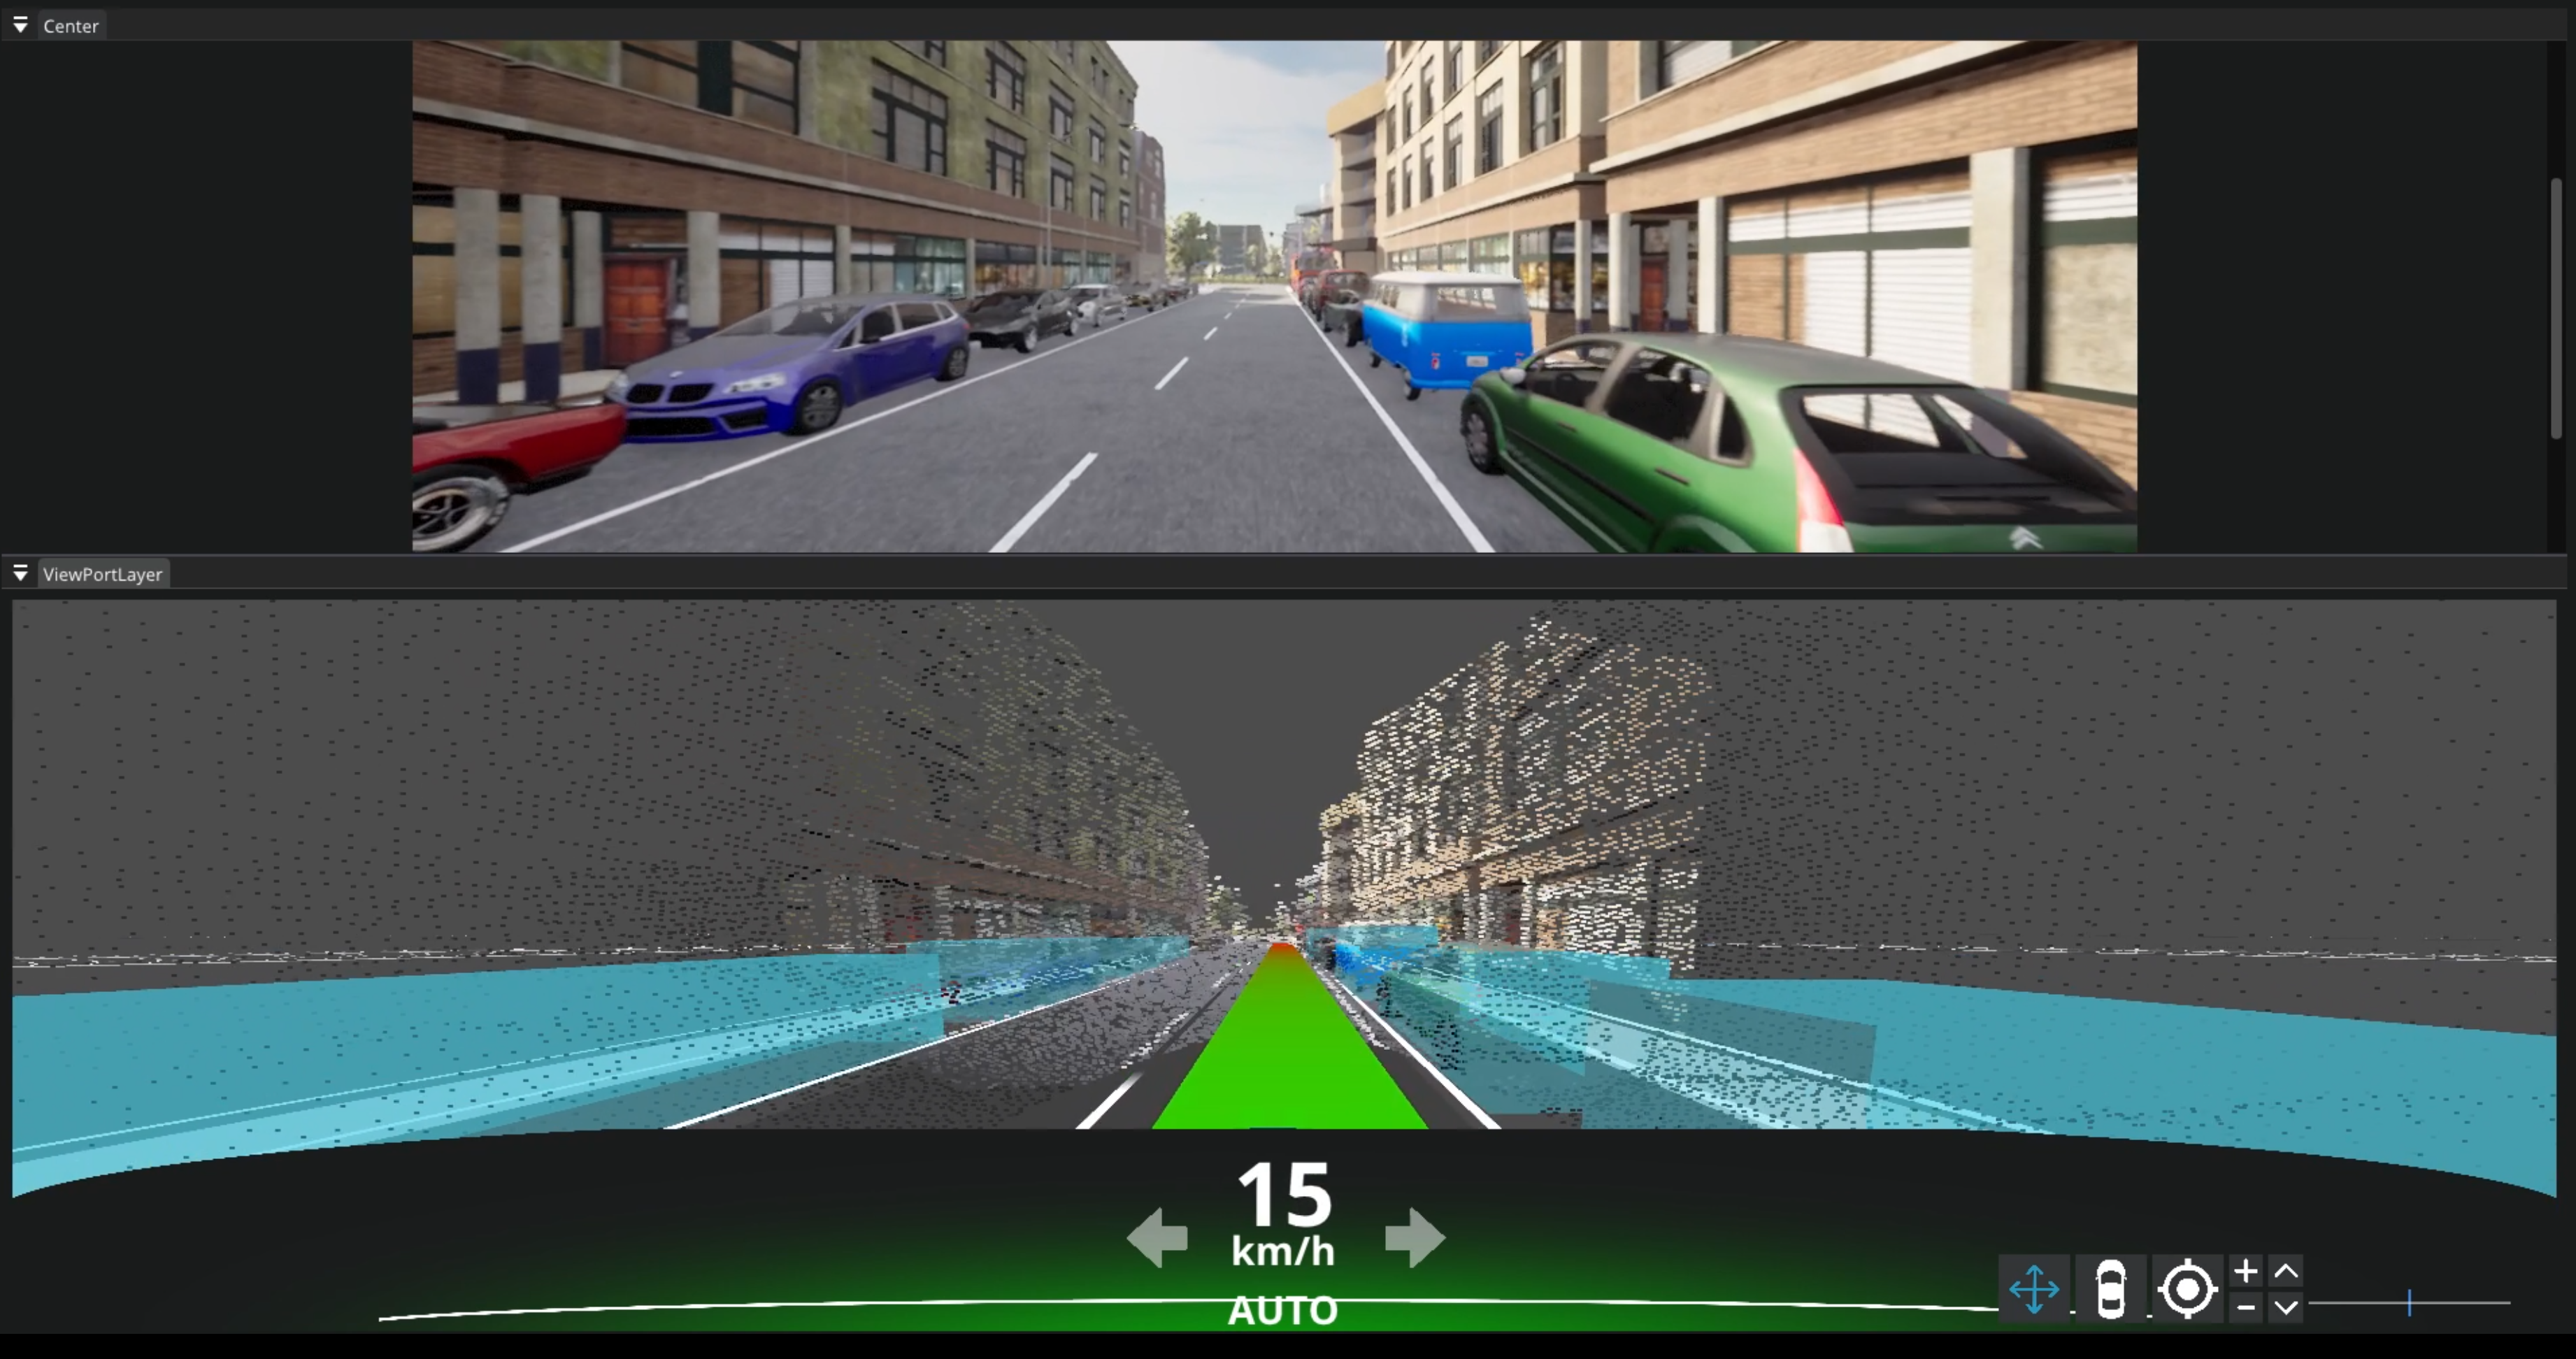
\includegraphics[width=\textwidth]{figures/results_2_sv.png}
        \centering
        \caption{Separate View Interface in a two sided street with parked vehicles}
        \label{fig:res_sv_2}
    \end{subfigure}
    \caption{Separate View Results}
    \label{fig:res_sv}
\end{figure}

\subsection*{Integrated View}

Integrated View is our novel approach to teleoperating interface design defined in the Section \ref{section:integratedview}.
The resulting visualization combining the 2D camera feed and 3D perception data by utilizing a depth completion model can be seen from the Figures \ref{fig:res_iv}.

This variant inherits certain limitations from its reliance on depth completion and training data. The performance notably degrades for environments not well represented in the training dataset. Additionally, as evident in Figure \ref{fig:res_iv_2}, the visualization quality diminishes for objects farther from the ego vehicle, with bounding boxes becoming less distinguishable compared to their representation in the Separate View (Figure \ref{fig:res_sv_2}).

Despite these limitations, the Integrated View offers a significant advantage by consolidating all information into a unified display. This consolidated approach provides an opportunity to evaluate the impact of single-window visualization versus multi-window approaches in teleoperation contexts. The integration of visual data streams into a single coherent view aims to reduce the cognitive load of switching between different displays while maintaining situational awareness.

\begin{figure}[h]
    \centering
    \begin{subfigure}{0.8\textwidth}
        \includegraphics[width=\textwidth]{figures/result_iv.png}
        \centering
        \caption{Integrated View Interface before a construction site}
        \label{fig:res_iv_1}
    \end{subfigure}
    \begin{subfigure}{0.8\textwidth}
        \includegraphics[width=\textwidth]{figures/results_2_iv.png}
        \centering
        \caption{Integrated View Interface in a two sided street with parked vehicles}
        \label{fig:res_iv_2}
    \end{subfigure}
    \caption{Integrated View Results}
    \label{fig:res_iv}
\end{figure}

\subsection*{Integrated View with Ground Truth Depth}
This variant utilizes CARLA's depth camera to obtain perfect depth information for visualization. By using ground truth depth data, it achieves the benefits of the Integrated View's unified visualization approach while avoiding the limitations of depth completion estimation. The interface maintains clear visibility of all objects, including those at greater distances, and provides accurate spatial relationships throughout the entire field of view. Such results can be seen from the Figures \ref{fig:res_gt_1} and \ref{fig:res_gt_2}.

The only technical limitation of this variant is the increased computational overhead due to the dense point-cloud requirements. However, this variant serves purely as a research tool for the user study, establishing an upper bound for visualization quality with perfect depth information. Thus we didn't undergo an in-depth optimization for the rendering process for this variant.

It's important to note that this implementation is not feasible for real-world deployment, as current depth sensing technology cannot provide sufficiently accurate for longer ranges in open environments (Table \ref{table:depth_camera_limitations}). Real-world depth cameras face significant limitations in accuracy and range, particularly under varying lighting conditions. Therefore, this variant primarily serves as a baseline for evaluating the potential of depth completion algorithms and unified visualization approaches.

\begin{figure}[h]
    \centering
    \begin{subfigure}{0.8\textwidth}
        \includegraphics[width=\textwidth]{figures/result_gt.png}
        \centering
        \caption{Integrated View Ground Truth Interface before a construction site}
        \label{fig:res_gt_1}
    \end{subfigure}
    \begin{subfigure}{0.8\textwidth}
        \includegraphics[width=\textwidth]{figures/results_2_gt.png}
        \centering
        \caption{Integrated View Ground Truth Interface in a two sided street with parked vehicles}
        \label{fig:res_gt_2}
    \end{subfigure}
    \caption{Integrated View Ground Truth Results}
    \label{fig:res_gt}
\end{figure}

\paragraph{Performance Analysis}
Runtime performance testing in crowded scenarios revealed significant differences between the three interface variants. The Separate View, processing approximately 18,000 points, achieved the fastest rendering time at 18ms. The Integrated View, despite handling 921,600 points, required 33ms for rendering, while the Ground Truth variant processed around 750,000 points in 52ms.

A detailed analysis of the Separate View's point cloud rendering pipeline revealed three main computational bottlenecks:

- Coordinate system transformation: 3ms

- Image plane projection: 5ms

- Adding points to the mesh and cropping: 5ms

The modular design of the Ground Truth and Separate View renderers performs these operations sequentially. In contrast, the \emph{Integrated View} Renderer benefits from first, having a depth image in the camera space, means it doesn't need some of the costly steps like coordinate system transformation and image plane projection. Those steps are handled within the model, and the model runs it's estimation's on parallel as defined in the Section \ref{section:performanceoptimization}
This optimization strategy proves highly effective, as the \emph{Integrated View} processes over fifty times more points than the Separate View while only requiring an additional 15ms of processing time.

\begin{table}[h!]
\centering
\begin{tabular}{|p{3.5cm}|p{3cm}|p{3cm}|p{3cm}|}
\hline
\textbf{Feature} & \textbf{Separate View} & \textbf{Integrated View} & \textbf{Integrated View GT} \\
\hline
Processing Time & 18ms & 33ms & 52ms \\
\hline
Point Cloud Size & ~18k points & 921.6k points & ~750k points \\
\hline
Update Frequency & Real-time & Near real-time & Real-time \\
\hline
\end{tabular}
\caption{Performance comparison of interface variants}
\label{table:interface_comparison}
\end{table}

It's important to note that these measurements focus solely on the point cloud rendering pipeline, excluding the parallel depth estimation process in the Integrated View. The performance metrics demonstrate that our optimization strategies successfully manage the increased computational demands of processing larger point clouds while maintaining acceptable runtime performance.
